
\begin{definition}{Recherche non-informée}{uninformed-search}
    La recherche \textbf{non-informée} est une stratégie de recherche qui n'utilise \textbf{pas}
    d'information sur l'état de l'environnement afin de le \textbf{guider} pour trouver une solution.
    Elle explore simplement l'espace de recherche de manière systèmatique. En utilisant souvent 
    des \textit{algorithmes} comme \textbf{DFS}, \textbf{BFS}.
\end{definition}

\begin{remark}\leavevmode
    La recherche non-informée est utilisée quand on ne connait pas l'état de l'environnement. 
    Lorsqu'on ne peut quantifier la qualité d'un état en utilisant des \textbf{informations heuristiques}
\end{remark}

\begin{definition}{Agent de Plannification}{planningagent}
    Les agents de plannification font des \textbf{hypothèses} sur les conséquences des actions entreprises
    et utilisent un \textbf{modèle} de l'environnement pour trouver un plan qui atteint son objectif.
\end{definition}

\underline{\textbf{Résolution de problèmes par la recherche}}:
\begin{enumerate}
    \item \textbf{Formulation de l'objectif}: L'agent doit avoir un objectif afin 
        de pouvoir organiser son comportement. Ca permet de limiter l'espace de recherche (\textit{actions entreprises})
    \item \textbf{Formulation du problème}: L'agent doit avoir un moyen de représenter les actions et les états 
        afin de pouvoir les manipuler
    \item \textbf{Recherche de la solution}: Avant d'agir dans le monde réel, l'agent  fait  une 
        simulation de séquences d'actions dans son modèle de l'environnement jusqu'à trouver un séquence 
        qui mène à l'objectif. C'est  la \textit{solution}
    \item \textbf{Exécution de la solution}: L'agent exécute la séquence d'actions dans le monde réel
\end{enumerate}

\begin{note}
    Un plan est une séquence d'actions qui mène à l'objectif.
\end{note}

\subsection{Problème de recherches} % (fold)
\label{sub:probleme_de_recherches}

\begin{definition}{Problème de Recherche}{searchprob}
    Un problème de recherche est défini par:
    \begin{itemize}
        \item \textbf{Ensemble d'État $S$}: Une situation dans lequel l'environnement peut être agencé
        \item \textbf{État initial $s_o$}: l'état dans lequel le problème commence
        % \item \textbf{Actions}: les actions possibles
        % \item \textbf{Transition}: la fonction qui définit les conséquences des actions
        \item \textbf{Actions $A(s)$}: les actions possibles dans l'état $s$
        \item \textbf{Modèle de Transition $Result(s, a)$}: la fonction qui définit les conséquences des actions. L'état résultant de l'action $a$ dans l'état $s$
        \item \textbf{État final}: l'état que l'on veut atteindre
        \item \textbf{Cout de l'action $c(s, a, s')$}: le coût de l'action $a$ dans l'état $s$ qui mène à l'état $s'$
        \item \textbf{Solution}: Une séquence d'actions qui mène de l'état initial à l'état final. La solution 
            peut être \textbf{optimale}, c'est à dire qu'il n'y a pas de solution dont le coût est moindre.
    \end{itemize}
\end{definition}

% Fais un graph pour illustrer la roumanie

\begin{figure}[H]
    \begin{center}
        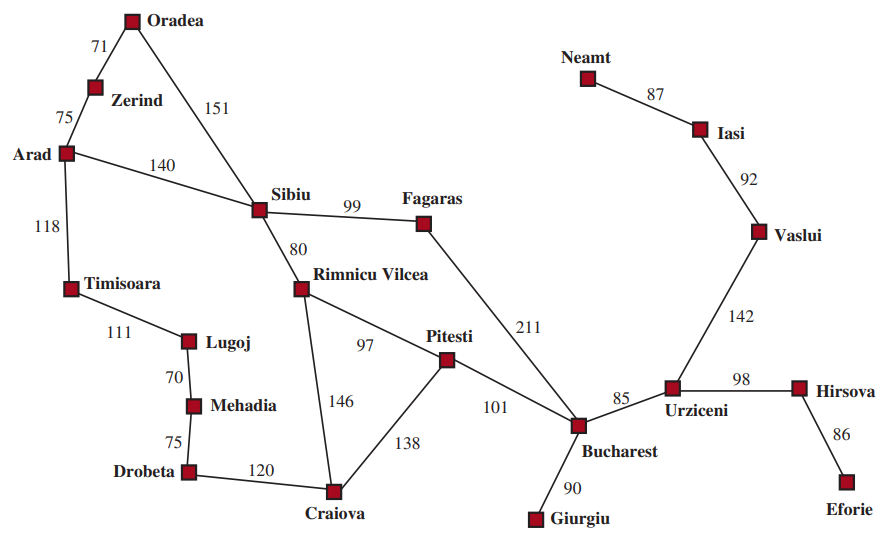
\includegraphics[width=0.70\textwidth]{./pictures/roumanie.png}
    \end{center}
    \caption{Représentation simple de la Roumanie en graphe}\label{fig:romania}
\end{figure}



\begin{example}\leavevmode
    Nous allons dés lors modéliser le problème de trouver un chemin entre deux villes en Roumanie.
    \begin{itemize}
        \item \textbf{États}: les villes de Roumanie
        \item \textbf{État initial}: Arad
        \item \textbf{Actions}: les routes entre les villes adjacentes
        \item \textbf{Modèle de transition}: Atteindre une ville adjacente
        \item \textbf{Cout de l'action}: distance entre les villes
        \item \textbf{État final}: Bucharest 
    \end{itemize}
\end{example}

% subsection Probleme de recherches (end)

\subsection{Graphe d'espace d'état} % (fold)
\label{sub:graphe_d_espace_d_etat}

\begin{definition}{Graphe d'espace d'état}{stategraph}
    Un graphe d'espace d'état est un graphe qui représente les états et les actions possibles.
    \begin{itemize}
        \item \textbf{Noeuds}: les états
        \item \textbf{Arêtes}: les résultats d'actions, successeurs
    \end{itemize} 
    L'état initial est le noeud racine et l'état final est un noeud (ou plusieurs ?).
    Les noeuds sont sont les représentations d'une configuration de l'environnement.
\end{definition}

\warningbox{Dans ce genre de graphe, chaque état n'est représenté qu'\textbf{une seule fois}.}

\begin{figure}[H]
    \begin{center}
        % 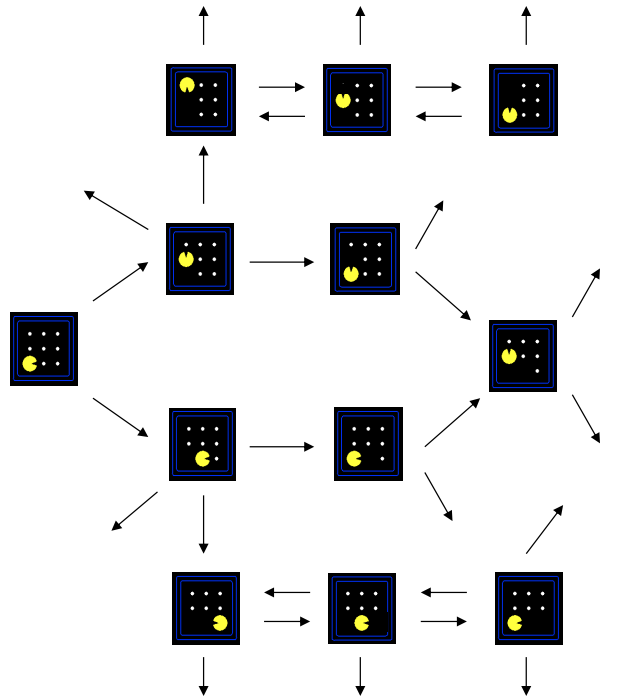
\includegraphics[width=0.45\textwidth]{../pictures/state_space_graph.png}
        \rotatebox{-90}{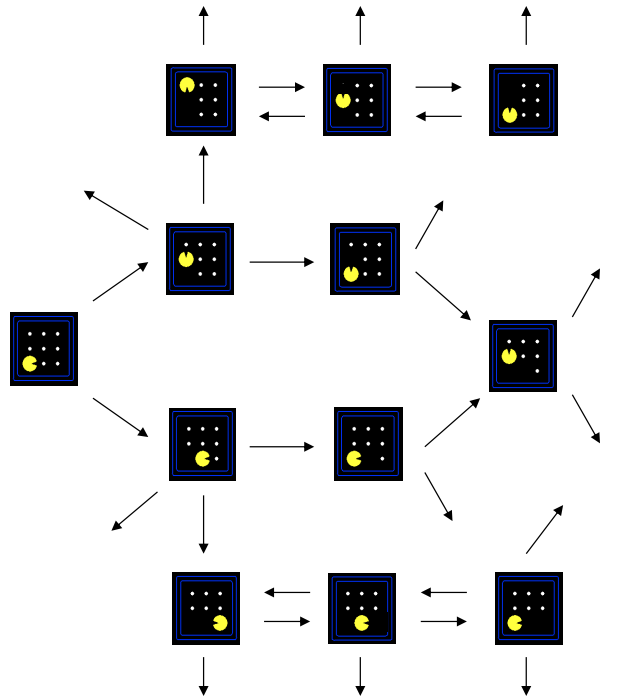
\includegraphics[width=0.45\textwidth]{../pictures/state_space_graph.png}}
    \end{center}
    \caption{Graph d'état partiel pour le jeu Pacman}\label{fig:stategraph}
\end{figure}


\begin{remark}\leavevmode
    Il est fortement possible de ne pas pouvoir représenter un problème de recherche par un graphe d'espace d'état car 
    il y a \textbf{trop d'états} ou que les états sont \textbf{continus}.
\end{remark}

% subsection Graphe d'espace d'etat (end)

\subsection{Arbres de Recherches} % (fold)
\label{sub:arbres_de_recherches}

\begin{definition}{Arbre de Recherche}{searchtree}
    Un arbre de recherche est un arbre qui représente les états et les actions possibles.
    C'est la représentation d'un \textit{Et si} je prenais cette action ? sur une certaine configuration de l'environnement.
    \begin{itemize}
        \item \textbf{Noeuds}: les états, plans pour arriver à ces états
        \item \textbf{Arêtes}: les actions
        \item \textbf{Enfants}: les états suivants (\textit{succeseurs})
    \end{itemize} 
    L'état initial est le noeud racine et l'état final est un noeud (ou plusieurs ?). 
    Les noeuds peuvent être représentés plusieurs fois, (\textbf{il est donc plus grand qu'un graphe d'espace d'état.})
\end{definition}


\begin{figure}[H]
    \begin{center}
        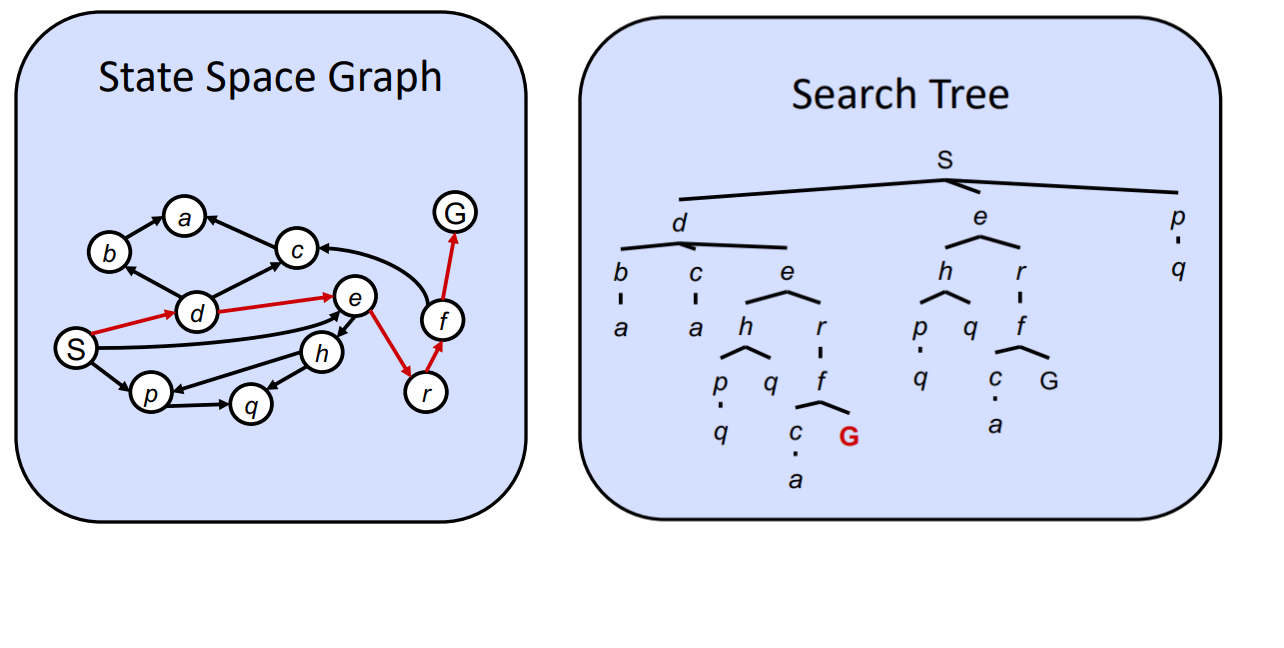
\includegraphics[width=0.5\textwidth]{../pictures/st_vs_sg.png}
    \end{center}
    \caption{Arbre de recherche vs Graphe d'espace d'état}\label{fig:stvssg}
\end{figure}

\warningbox{
    Chaque noeuds dans un arbre de recherche, est un chemin dans le graphe d'espace d'état.
}

\begin{note}
    L'arbre de recherche est construit au \textbf{fur et à mesure} de la recherche. 
    En général, on essaye de  minimiser sa taille.
\end{note}



\begin{figure}[H]
    \begin{center}
        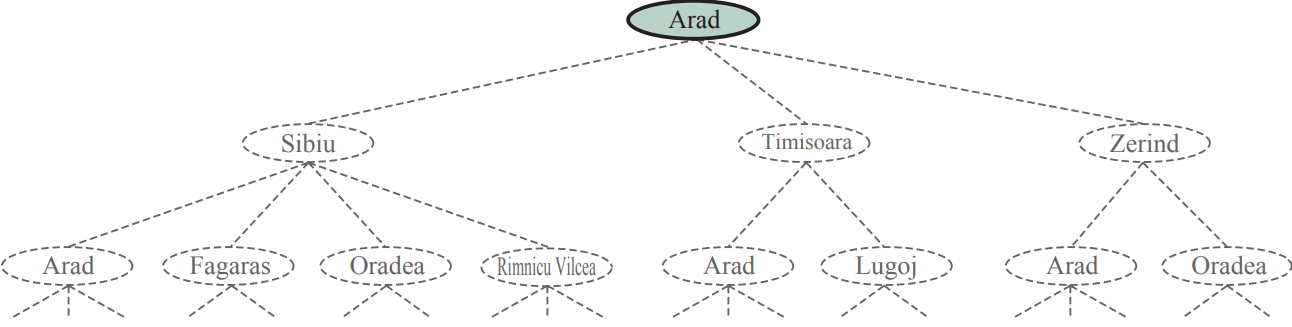
\includegraphics[width=0.75\textwidth]{./pictures/romst.png}
    \end{center}
    \caption{Arbre de recherche de la figure \ref{fig:romania}}\label{fig:romst}
\end{figure}

\subsubsection{Recherche dans un arbre de recherche} % (fold)
\label{sec:recherche_dans_un_arbre_de_recherche}

\begin{algorithm}[H]
    \floatname{algorithm}{Recherche dans un Arbre}
    \caption{Algorithme de recherche}\label{alg:stsearch}
    \begin{algorithmic}
        \Function{Tree-Search}{problème, stratégie} 
        \State initialise un noeud avec l'état initial du problème

        \Loop{
            \If{il ne peut plus y avoir d'état à explorer}
                \State \Return Erreur
            \EndIf
            \State choisis un noeud non exploré selon la stratégie
            \If{le noeud est l'état final}
                \State \Return le plan qui mène à l'état final
            \Else
                \State Développe le noeud et ajoute ses enfants à l'arbre
            \EndIf
        }
        \EndLoop
        \EndFunction
    \end{algorithmic}
\end{algorithm}

\begin{remarks}\leavevmode
\begin{enumerate}
    \item La frontière est l'ensemble des noeuds construits non explorés de l'arbre
    \item Pour développer un noeud de la frontiere, on le retire de la frontière et on l'ajoute à l'ensemble des noeuds explorés
        ses enfants sont ajoutés à la frontière
    \item La recherche dans un graphes est similaire à la recherche dans un arbre sauf qu'on doit vérifier si un noeud a déjà été visité
        avant de l'ajouter à la frontière
\end{enumerate}
\end{remarks}

% subsubsection Recherche dans un arbre de recherche (end)

% subsection Arbres de Recherches (end)

\begin{figure}[H]
    \begin{center}
        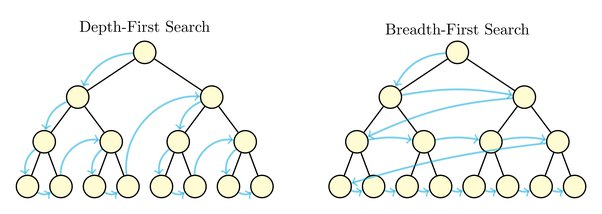
\includegraphics[width=0.95\textwidth]{./pictures/bfsschema.jpg}
    \end{center}
    \caption{Sens d'éxécution BFS et DFS}\label{fig:bfsschema}
\end{figure}



\subsection{Depth-First Search (DFS)} % (fold)
\label{sub:dfs}

\begin{definition}{DFS}{dfs}
    La recherche en profondeur (\textbf{DFS}) est une stratégie de recherche qui explore l'arbre en allant le plus loin possible dans une branche avant de revenir en arrière. 
    \begin{itemize}
        \item \textbf{Frontière}: une pile (LIFO)
        \item \textbf{Stratégie}: on choisit le noeud le plus profond de la frontière et on l'étend
    \end{itemize} 
\end{definition}
% subsection DFS (end)

\subsection{Breadth-First Search (BFS)} % (fold) 
\label{sub:bfs} 

\begin{definition}{BFS}{bfs}
    La recherche en largeur (\textbf{BFS}) est une stratégie de recherche qui explore l'arbre en allant le plus large possible dans une branche avant de revenir en arrière. 
    \begin{itemize}
        \item \textbf{Frontière}: une file (FIFO)
        \item \textbf{Stratégie}: on choisit le noeud le moins profond de la frontière et on l'étend
    \end{itemize} 
\end{definition} 
% subsection BFS (end)

\textbf{DFS} est meilleur que \textbf{BFS} dans les cas suivant: 
\begin{itemize}
    \item Si il y a des limitations de mémoire 
\end{itemize}

\textbf{BFS} est meilleur que \textbf{DFS} dans les cas suivant: 
\begin{itemize}
    \item Si on veut trouver la solution la plus courte
\end{itemize}

\subsection{Iterative deepening} % (fold)
\label{sub:iterative_deepening}
\begin{note}
    L'idée est d'avoir les avantages mémoire de \textbf{DFS} et la solution optimale de \textbf{BFS}
\end{note}

\begin{definition}{Iterative deepening}{iterdeep}

    L'exploration itérative en profondeur (\textbf{Iterative deepening}) est une stratégie de 
    recherche qui explore l'arbre en faisant une recherche en profondeur avec une limite de profondeur de 
    1, puis 2, puis 3, etc. jusqu'à ce que la solution soit trouvée.


    % TODO: Se renseigner sur ça 
    % L'exploration itérative en profondeur (\textbf{Iterative deepening}) est une stratégie de recherche qui explore l'arbre en allant le plus loin possible dans une branche avant de revenir en arrière. 
    % \begin{itemize}
    %     \item \textbf{Frontière}: une pile (LIFO)
    %     \item \textbf{Stratégie}: on choisit le noeud le plus profond de la frontière
    % \end{itemize} 
\end{definition}

\begin{remark}\leavevmode
    Même si cette algorithme visite plusieurs fois les mêmes noeuds, ça n'a pas vraiment d'impact
    car le nombre de noeuds est réduit. En effet, on mise de le trouver avant d'atteindre la limite de profondeur. 
    Plus on avance dans l'arbre, plus le nombre de noeuds augmente de $b$ (branching factor), nous misons donc sur le fait que la solution se trouve dans les premiers noeuds.
\end{remark}

% subsection Iterative deepening (end)


\subsection{UCS} % (fold) 
\label{sub:ucs} 

\begin{definition}{Uniform Cost Search}{ucs}
    La recherche par coût uniforme (\textbf{UCS}) est une stratégie de recherche qui explore l'arbre en allant le plus loin possible dans une branche avant de revenir en arrière. 
    \begin{itemize}
        \item \textbf{Frontière}: une file de priorité
        \item \textbf{Stratégie}: on choisit le noeud ayant le plus petit coût de la frontière
    \end{itemize} 
\end{definition} 




Pour ananlyser un algorithme, on va utilser ces différentes propriétés:
\begin{itemize}
    \item \textbf{Complet}: l'algorithme trouve toujours une solution si elle existe
    \item \textbf{Optimal}: l'algorithme trouve toujours la solution optimale (avec le plus petit coût)
    \item \textbf{Complexité en temps}: Combien de temps l'algorithme prend pour trouver une solution
    \item \textbf{Complexité en espace}: Combien de mémoire l'algorithme prend pour trouver une solution
\end{itemize}

\begin{table}[H]
    \caption{Comparaison stratégie d'exploration}\label{tab:searchcomp}
    \begin{center}
        \begin{tabular}[c]{|l||l|l|l|l|}
            \hline
            \multicolumn{1}{|c|}{\textbf{Critère}} & 
            \multicolumn{1}{|c|}{\textbf{Largeur}} &
            \multicolumn{1}{c|}{\textbf{Cout uniforme}} &
            \multicolumn{1}{c|}{\textbf{Profondeur}} &
            \multicolumn{1}{c|}{\textbf{Profondeur itérative}} \\

            \hline
            \textbf{Complet}& Oui & Oui & Non (cycle, $\infty$ noeuds) & Oui \\ 
            \hline
            \textbf{Optimal}& Oui & Oui & Non & Oui\\ 
            \hline
            \textbf{Temps}& $O(b^d)$ & $O(b^{\frac{C^*}{\epsilon}})$ & $O(b^m)$ & $O(b^d)$\\ 
            \hline
            \textbf{Espace}& $O(b^d)$ & $O(b^{\frac{C^*}{\epsilon}})$ & $O(bm)$ & $O(bd)$\\

            \hline
        \end{tabular}
    \end{center}
\end{table}
